\documentclass[a4paper]{article}

\usepackage{fullpage} % Package to use full page
\usepackage{parskip} % Package to tweak paragraph skipping
\usepackage{tikz} % Package for drawing
\usepackage{amsmath}
\usepackage{hyperref}

\title{MTH 4300: Algorithms, Computers, and Programming II}
\author{Spring 2025}
\date{Midterm Review}

\begin{document}
\maketitle


\section{TRUE OR FALSE}
\begin{enumerate}
    \item The command to compile and rename a file is: g++ main.cpp -o main
    \item the literal "apple" is an lvalue 
    \item the float data type can \textbf{only} store positive integers 
    \item while loops are used when you need a program to loop, 
          and the number of times it will loop is detetmined at run time.
    \item Is this syntax correct: int matrix[3][3] = \{1, 2, 3\},\{4, 5, 6\},\{7, 8, 9\};
    \item Base case for recursion is always required
    \item Arrays are technically pointers
    \item new is used to mark an item as never seen before
    \item Passing by reference allows you to avoid copying an object, improving performance, but returning
    by value ensures the caller receives a new copy of the object.
    \item All variables on the heap must be referenced using pointers
\end{enumerate}
\newpage


\section{SHORT ANSWER}
\begin{enumerate}
    \item What is the downside of storing variables in the function call stack?
    \item What is the terminal command to create a new folder?
    \item Fix the function below: 
    \begin{verbatim}
        void my_function(int param1, param2)
        {
          cout<"hello"<<endl;
          return 7;
        }
    \end{verbatim}
          
    \item initialization list must be used if one of your attributes is a reference variable.
    \item What does the sizeof function return ?
    \item Whats a disadvantage of recursion?
    \item Consider the function signature \textbf{void func(int alpha, int beta=9, int gamma)}, is the syntax correct ?
    \item Whats a dangling pointer and how is it caused.
    \item does int* const ptr; make the address stored or the content of the address stored const?
    \item The variable int* pointer = \&x; is stored on the heap or the stack?
\end{enumerate}
\newpage 


\section{CODING(midterm will only have 2 questions here)}
\begin{enumerate}
    \item Write a c++ class to describe a toaster. Make sure to include at least
          3 attributes(set to private), 3 methods(set to public), and a 
          constructor(set to public). Write a main function and create 2 objects in the main. Figure out a way to print one 
          of your attributes in the main by calling one of your methods.
    \item Write a main function that creates a 5 by 5, 2d integer array(on the heap or 
          stack whatever you prefer). Then prompt the user to enter a row number x, and a value y. 
          For row x, fill up each entry with (y + column number).
    \item What does the following code print:
    \begin{verbatim}
        int x = 10;
        int* y = &x;
        x=17;
        *y=22;
        cout<<x<<endl;
    \end{verbatim}
    \item What does the following code print:\\
    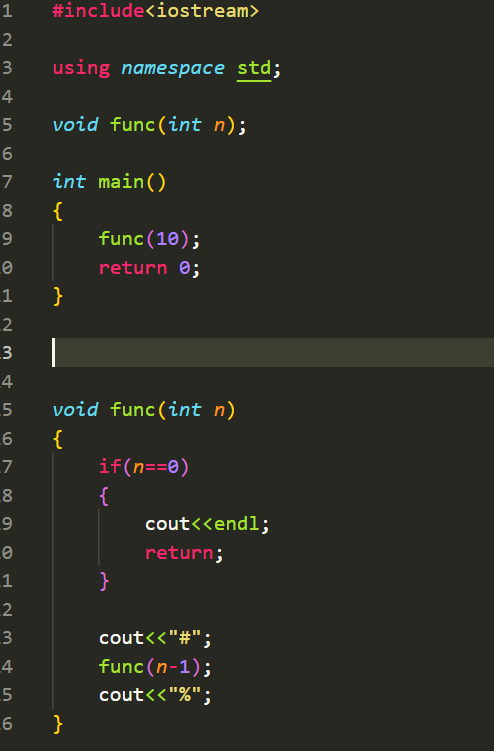
\includegraphics[width=5cm]{question2.png}
    
\end{enumerate} 
\newpage

\section{SOLUTIONS}
\subsection{TRUE OR FALSE}
\begin{enumerate}
    \item true
    \item false
    \item false
    \item true
    \item false
    \item true
    \item true
    \item false
    \item true
    \item true
\end{enumerate}

\subsection{SHORT ANSWER}
\begin{enumerate}
    \item it can get full and you are not allowed to resize it
    \item mkdir
    \item \begin{verbatim}
            int my_function(int param1,int param2)
            {
            cout<<"hello"<<endl;
            return 7;
            }
            \end{verbatim}
    \item yes
    \item the number of bytes for the type of the input variable
    \item It can cause a stack overflow, too much overhead for simpler problems
    \item default arguments are incorrect
    \item When a pointer points to memory that has been freed. It is caused after
          you use the delete operator and forget to set the ptr to nullptr.
    \item address stored
    \item stack
\end{enumerate}

\subsection{CODING(files below located inside this repo)}
\begin{enumerate}
    \item \href{run:./review_coding_question1.cpp}{review\_coding\_question1.cpp}
    \item \href{run:./review_coding_question2.cpp}{review\_coding\_question2.cpp}
    \item \href{run:./review_coding_question3.cpp}{review\_coding\_question3.cpp}
    \item \href{run:./review_coding_question4.cpp}{review\_coding\_question4.cpp}
\end{enumerate}

\end{document}